\documentclass{article}

\usepackage{hyperref}
\usepackage[T1]{fontenc}
\usepackage{graphicx}
\usepackage{float}
\usepackage[utf8]{inputenc}
\usepackage{amsmath}


\title{%
Laboratorium 8\\
  \huge Rozwiązywanie równań nieliniowych}
\author{Mateusz Król}
\date{07/05/2024 r.}

\begin{document}
\maketitle

 
\section*{Zadanie 1.}
\textbf{Dla poniższych funkcji i punktów początkowych metoda 
\textit{Newton}'a
zawodzi. Wyjaśnij dlaczego. Następnie znajdź pierwiastki.
$$f_1(x) = x^3-5x,\ x_0=1$$
$$f_2(x) = x^3-3x+1,\ x_0=1$$
$$f_3(x) = 2-x^5,\ x_0=0.01$$
$$f_4(x) = x^4-4.29x^2-5.29,\ x_0=0.8$$} \\
\null\quad
Wykorzystałem funkcję \textit{scipy.optimize.newton} z modułu
\textit{SciPy}. \\\\
Dla funkcji $f_1$ metoda \textit{Newton}'a działa - zwraca prawdziwy
pierwiastek ($\approx 4.7 \cdot 10^{-24} \approx 0$). W celu zwrócenia
innego pierwiastka, możnaby zmienić wartość początkową na bliższą
odpowiedniej wartości (np. $2$). \\\\
Dla reszty funkcji metoda \textit{Newton}'a nie działa: \\\\
Dla funkcji $f_2$ odpowiednim $x_0$ byłoby $1.5$, gdyż wartość $1$ jest
ekstremum lokalnym. \\
Dla funkcji $f_3$ lepszym wyborem $x_0$ byłoby $1.1$, gdyż metoda \textit{scipy.optimize.newton},
niezależnie od przekazanej do funkcji parametru liczby iteracji, stale pozostaje w punkcie 0.01. \\
Innym rozwiązaniem jest przekazanie do funkcji wartości parametru \textit{tol} o przykładowej
wartośći 0.01. \\
Dla funkcji $f_3$ odpowiednim $x_0$ byłoby $2.0$ - wartość bliżej 
prawdziwego pierwiastka. \\\\

\section*{Zadanie 2.}
\textbf{Dane jest równanie: $$f(x)=x^2-3x+2=0$$
Każda z następujących funkcji definiuje równoważny schemat iteracyjny:
$$g_1(x)=\frac{(x^2+2)}{3}$$
$$g_2(x)=\sqrt[]{3x-2}$$
$$g_3(x)=3-\frac{2}{x}$$
$$g_4(x)=\frac{(x^2-2)}{2x-3}.$$
}
\\\\
\null\quad Funkcje pochodne funkcji $g_i(x)$:
$$g_1(x)=\frac{2x}{3}$$
$$g_2(x)=\frac{3}{2\cdot \sqrt[]{3x-2}}$$
$$g_3(x)=\frac{2}{x^2}$$
$$g_4(x)=\frac{2(x^2-3x+2)}{(2x-3)^2}$$

Tabela z wartościami rzędów zbieżności schematów iteracyjnych 
odpowiadających funkcjom $g_i$:
\begin{center}
  \begin{tabular}{c c} 
   Function & Order of convergence\\
   $g_1$ & $\approx 1.33$\\
   $g_2$ & $0.75$\\
   $g_3$ & $0.5$\\
   $g_4$ & $0$
  \end{tabular}
\end{center}
Wykres przedstawiający porównanie wartości błędów względnych w zależności od liczby
iteracji:
\begin{figure}[H]
  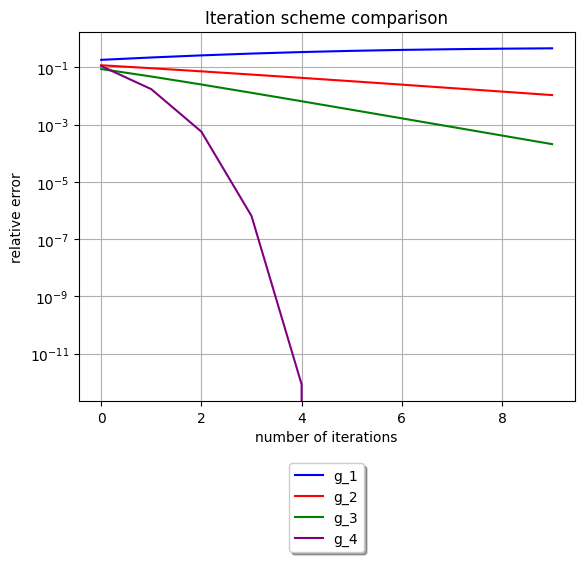
\includegraphics[width=\linewidth]{figures/iteration.png}
\end{figure}

Wartości bezwględne pochodnych funkcji: $g_2$, $g_3$, $g_4$ w punkcie $x_0=2$, wynoszą mniej od 1, z czego
powinna wynikać zbieżność odpowiadających im schematów iteracyjnych,
co pokrywa się z danymi odczytanymi z wykresu. \\\\
\null\quad
Wartość pochodnej $g_4$ w punkcie $x_0$ wynosi 0, co świadczy o conajmniej kwadratowej zbieżności
schematu iteracyjnego, co zgadza się z obliczoną wartością rzędu zbieżności $\approx 1.9997$.



\section*{Zadanie 3.}
\textbf{Napisz schemat iteracji wg metody Newtona dla każdego z nastę-
pujących równań nieliniowych:
$$x^3-2x-5=0$$
$$e^{-x} = x$$
$$x\cdot\sin(x) = 1$$}

\begin{figure}[H]
  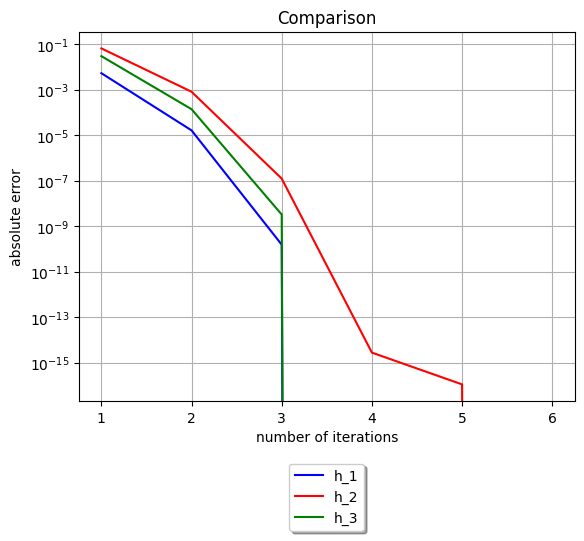
\includegraphics[width=\linewidth]{figures/comparison.png}
\end{figure}

Metoda \textit{Newton}'a posiada kwadratowy rząd zbieżności, więc za każdą iteracją,
wartość błędu dwukrotnie maleje, a co za tym idzie, dokładność na kolejnych bitach zwiększa się dwukrotnie.\\
Można to również wywnioskować na podstawie zamieszczonego wykresu.

\section*{Zadanie 4.}
\textbf{Napisz schemat iteracji wg metody Newtona dla następującego
układu równań nieliniowych:
$$x_1^2 + x_2^2 = 1$$
$$x_1^2 - x_2 = 0$$}

Wykres przedstawiający wartości błędu względnego obliczego rozwiązania
układu równań, w zależności od liczby iteracji:
\begin{figure}[H]
  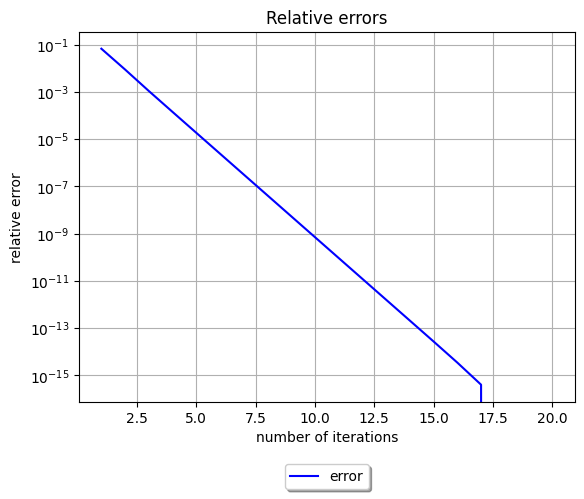
\includegraphics[width=\linewidth]{figures/multivariable.png}
\end{figure}

\end{document}